\documentclass{article}
\usepackage[backend=biber,natbib=true,style=alphabetic,maxbibnames=50]{biblatex}
\addbibresource{/home/nqbh/reference/bib.bib}
\usepackage[utf8]{vietnam}
\usepackage{tocloft}
\renewcommand{\cftsecleader}{\cftdotfill{\cftdotsep}}
\usepackage[colorlinks=true,linkcolor=blue,urlcolor=red,citecolor=magenta]{hyperref}
\usepackage{amsmath,amssymb,amsthm,float,graphicx,mathtools,tikz}
\usetikzlibrary{angles,calc,intersections,matrix,patterns,quotes,shadings}
\allowdisplaybreaks
\newtheorem{assumption}{Assumption}
\newtheorem{baitoan}{Bài toán}
\newtheorem{cauhoi}{Câu hỏi}
\newtheorem{conjecture}{Conjecture}
\newtheorem{corollary}{Corollary}
\newtheorem{dangtoan}{Dạng toán}
\newtheorem{definition}{Definition}
\newtheorem{dinhly}{Định lý}
\newtheorem{dinhnghia}{Định nghĩa}
\newtheorem{example}{Example}
\newtheorem{ghichu}{Ghi chú}
\newtheorem{hequa}{Hệ quả}
\newtheorem{hypothesis}{Hypothesis}
\newtheorem{lemma}{Lemma}
\newtheorem{luuy}{Lưu ý}
\newtheorem{nhanxet}{Nhận xét}
\newtheorem{notation}{Notation}
\newtheorem{note}{Note}
\newtheorem{principle}{Principle}
\newtheorem{problem}{Problem}
\newtheorem{proposition}{Proposition}
\newtheorem{question}{Question}
\newtheorem{remark}{Remark}
\newtheorem{theorem}{Theorem}
\newtheorem{vidu}{Ví dụ}
\usepackage[left=1cm,right=1cm,top=5mm,bottom=5mm,footskip=4mm]{geometry}
\def\labelitemii{$\circ$}
\DeclareRobustCommand{\divby}{%
	\mathrel{\vbox{\baselineskip.65ex\lineskiplimit0pt\hbox{.}\hbox{.}\hbox{.}}}%
}

\title{Problem: Thal\`es Theorem -- Bài Tập: Định Lý Thal\`es}
\author{Nguyễn Quản Bá Hồng\footnote{Independent Researcher, Ben Tre City, Vietnam\\e-mail: \texttt{nguyenquanbahong@gmail.com}; website: \url{https://nqbh.github.io}.}}
\date{\today}

\begin{document}
\maketitle
\tableofcontents

%------------------------------------------------------------------------------%

\begin{dinhly}[Thal\`es]
	Cho $\Delta ABC$. Nếu 2 điểm $E,F$ lần lượt nằm trên cạnh $CA,AB$ sao cho $EF\parallel BC$ thì $\dfrac{AE}{AC} = \dfrac{AF}{AB} = \dfrac{EF}{BC}$.
\end{dinhly}

\begin{dinhly}[Thal\`es đảo]
	Cho $\Delta ABC$. Nếu 2 điểm $E,F$ lần lượt nằm trên cạnh $CA,AB$ sao cho $\dfrac{AE}{AC} = \dfrac{AF}{AB} = \dfrac{EF}{BC}$ thì $EF\parallel BC$.
\end{dinhly}

\begin{center}
	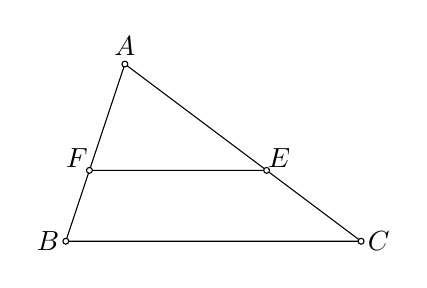
\begin{tikzpicture}[scale=.75]
		\path
		(1,3) coordinate (A)
		(0,0) coordinate (B)
		(5,0) coordinate (C)
		($(A)!.6!(C)$) coordinate (E)
		($(A)!.6!(B)$) coordinate (F);
		\draw (A)--(B)--(C)--cycle (E)--(F);
		\foreach \x/\g in {A/90,B/180,C/0,E/45,F/135} \draw[fill=white] (\x) circle (.05) + (\g:.3) node{$\x$};
	\end{tikzpicture}
\end{center}

\begin{baitoan}[\cite{Hung_Dung_Mai_Qua_Long_Toan_9_hinh_hoc}, 1., p. 6, Sharygin 2015]
	$BM$ là đường trung tuyến của tam giác vuông không cân $ABC$, vuông tại B \& $H_a,H_c$ tương ứng là trực tâm $\Delta ABM,\Delta CBM$. $AH_c,CH_a$ cắt nhau tại K. Chứng minh $\widehat{MBK} = 90^\circ$.
\end{baitoan}

\begin{baitoan}[\cite{Hung_Dung_Mai_Qua_Long_Toan_9_hinh_hoc}, 2., p. 6, Sharygin 2016]
	$AH_1,BH_2$ là 2 đường cao của $\Delta ABC$ nhọn, D là hình chiếu của $H_1$ trên AC, E là hình chiếu của D trên AB, F là giao điểm của ED \& $AH_1$. Chứng minh $H_2F\parallel BC$.
\end{baitoan}

\begin{baitoan}[\cite{Hung_Dung_Mai_Qua_Long_Toan_9_hinh_hoc}, 3., p. 7]
	Cho tứ giác $ABCD$ \& 2 điểm $E,F$ tương ứng thuộc 2 đoạn $AB,CD$ sao cho $\dfrac{EA}{EB} = \dfrac{FD}{FC}$. Chứng minh các điểm chia trong 3 đoạn thẳng $AD,BC,EF$ theo cùng 1 tỷ số thẳng hàng.
\end{baitoan}

%------------------------------------------------------------------------------%

\section{Miscellaneous}

%------------------------------------------------------------------------------%

\printbibliography[heading=bibintoc]
	
\end{document}